\chapter{Appendix A}\label{appendix-a}

\section{Modelling of flow and
transport}\label{modelling-of-flow-and-transport}

\subsection{Molecular diffusion}\label{molecular-diffusion}

As emphasized by \citep[p194]{Battjes2017}: ``..molecular diffusion is
irrelevant in civil engineering practice, where turbulent diffusion and
dispersion are dominant..''.

In this case however it could be relevant because of the specific
experiment. Still with the goal of modelling the Rhine-Maas delta in
mind emphasis may be put on diffusion and dispersion processes related
to turbulence.

\subsection{Turbulent diffusion}\label{turbulent-diffusion}

To describe the turbulent diffusion the fluctuating quantities are
averaged over a certain time and lenght scale. Because of gravity the
concentration gradient is positive in the downward z-direction. From the
averaging of the turbulent motion and the gravity induced concentration
gradient it follows, as quoted from \citep[p.197]{Vuik2007}, that:
``..turbulent fluctuations cause a mean transport in the direction of
decreasing values of the mean concentration, as in a diffusion
process.''

Because the fluctuating quantities cause such net transport processes,
the resulting motion and turbulent properties need to be quantified. To
this end \citet{Prandtl1925} defined the concept of mixing lenght that
defines the lenght over which the fluctuations cause a deviation from
the average state and correspond to the average distance the turbulence
eddies travel. For example, velocity fluctuations can be related to the
velocity of the turbulent eddies. Further the turbulence induced
transport processes are found to be proportional to the concentration
gradient, also called the turbulence diffusivity. It has the order of
magnitude of the eddie velocity times the mixing lenght.

For vertical diffusion in free surface flows the mixing lenght changes
over the depth since it is induced by the bed friction expressed in the
bed shear stress (τ-b). Using his an estimate of the particle velocity
can be made by the so-called shear velocity which together with a
parabolic variation of the mixing length over the depth gives a measure
for the turbulence diffusivity: εt = Κ∙u∙L = Κ∙u∙z∙(1 - z/d). Where Κ is
the Von Karman coefficient which was previously empirically determined.

In exactly this manner horizontal momentum can be vertically distributed
through so-called Reynolds shear stress (τ-xz). Thus, in this case it is
not a concentration (c) but a momentum per unit volume (ρu) that is
diffused, an effect referred to as eddy viscosity. In a simple free
surface flow \citep[p.199]{Vuik2007} shows how this leads to a
logarithmic velocity profile.

\section{Turbulence modelling in D-Flow
FM}\label{turbulence-modelling-in-d-flow-fm}

\subsection{Reynold stresses}\label{reynold-stresses}

In the D-Flow FM model the total horizontal viscosity can be divided
into three contributing parts: - sub grid scale turbulence - 3D
turbulence - dispersion for depth averaged simulation

\subsubsection{Horizontal eddy
viscosity}\label{horizontal-eddy-viscosity}

Modelling horizontal eddy viscosity has three seperate parameters that
determine the total viscosity as follow: μ-H = μ-sgs + μ-v + μ-H-back.

These three parameters account for the following: - Horizontal turbulent
viscosity may be underestimated because of the sub-grid scale turbulent
motions, i.e.~turbulence on a scale smaller than the meshgrid. This can
be resolved by the sub-grid scale viscosity: μ-sgs - With Reynolds
averaged shallow water equations horizontal eddy viscosity might not
accounted for (enough) either thus D-Flow introduces the μ-v. - If extra
constant or spatially dependant viscosity is desired the background
viscosity μ-back may be added.

With respect to the 3D viscosity resulting from three-dimensional
turbulence a closure model is used \citep[p.26]{DFlowTechMan}. For
specific closure models one can even account for unresolved mixing
through an ambient background mixing coefficient μ-V-back. Eventually
the vertical eddy viscosity is thus calculated by a combination of the
3D viscosity μ-v and μ-mol, the latter being the kinematic viscosity of
water, as follows: μ-v = μ-mol + max(μ-v, μ-v-back).

In D-Flow FM four turbulence closure models can be chosen, the first
being user defined and the latter three based on models by Kolmogorov
and Prandtl, all are explained in further detail in
\citep[p.112-120]{DFlowTechMan}; - Constant coefficient - resulting in a
parabolic vertical velocity profile - Algebraic eddy viscosity closure
model - based on the Von Karman constant (κ), the bed friction (Cf),
without including transport processes, computing mixing lenght (L), the
shear velocity and the vertical turbulent viscosity μ-v. - Κ-ε
turbulence model - involves solving a non-linear coupled system of
equations describing turbulent kinetic energy (Κ) and energy loss (ε)
including diffusivity coefficients (D), a turbulent kinetic energy
production term (P), a Buoyancy flux (B) and a variation of kalibration
terms (c1-3). Thereafter the vertical eddy viscosity μ-v is determined
as proportional to the ratio Κ²/ε and the mixing lenght. Still, this
coupled system has to be discretized in terms of advection and diffusion
which is done explicitly by a first order upwind scheme and implicitly,
respectively. Accordingly the production and buoyancy term are
discretized while conserving the diagonally dominant matrix (ensuring
positivity). Finally this leads to two tri-diagonal matrices for Κ and ε
that can be solved using Thomas algorithm, which may be seen as the
tri-diagonal LU-decomposition, by using specific boundary conditions. -
Κ-τ turbulence - Where τ is a typical timescale of the turbulent eddies
and the eddy viscosity is proportional to Κ∙τ. Coupled by a system of
convection diffusion equations including diffusivity, production and
buoyancy terms. The resulting advection equation is discretized with an
first order upwind difference scheme and the vertical diffusion term is
discretized implicitly by a temporal discretization scheme. Again this
leads to two tri-diagonal matrices that can be solved by the Thomas
algorithm using specific boundary conditions.

\chapter{Appendix B}\label{appendix-b}
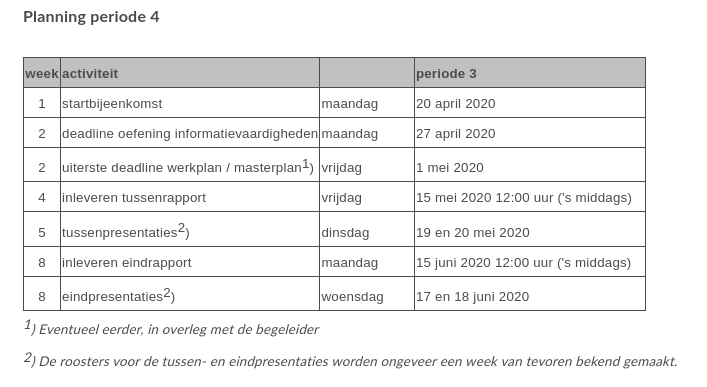
\includegraphics{/mnt/c/Users/daank/civiel/BEP/working/planofaction/planning.png}
